\documentclass[12pt]{article}
\usepackage[margin=1in]{geometry}
\usepackage{amsmath,amssymb}
\usepackage{booktabs}
\usepackage{graphicx}
\usepackage{subcaption}
\graphicspath{{figures/}}
\usepackage[colorlinks=true,linkcolor=blue]{hyperref}

% Same macros as main.tex
\newcommand{\Vac}{\mathrm{V}}          % vacancy
\newcommand{\Int}{\mathrm{I}}          % self-interstitial
\newcommand{\GB}{\mathrm{GB}}
\newcommand{\eq}{\mathrm{eq}}
\newcommand{\eff}{\mathrm{eff}}
\newcommand{\intf}{\mathrm{int}}       % interface
\newcommand{\thr}{\mathrm{th}}         % threshold
\newcommand{\lat}{\mathrm{lat}}
\newcommand{\ox}{\mathrm{ox}}
\newcommand{\Ox}{\mathrm{O}}           % oxygen


\usepackage[
  backend=biber,
  style=numeric-comp,
  sorting=none
]{biblatex}

\addbibresource{refs/ref.bib}

\title{mode revision note}


\begin{document}
\maketitle

\section*{finite sink for GB}

\begin{figure}[!ht]\centering
\begin{subfigure}[t]{0.32\textwidth}\centering
  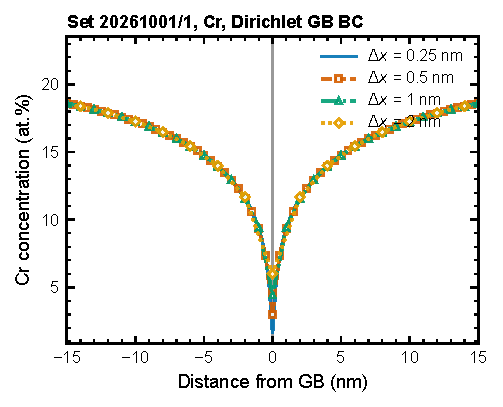
\includegraphics[width=\linewidth]{Cr_Dirich_vs_dx}
  \caption{}\label{fig:Cr-Dirich}
\end{subfigure}\hfill
\begin{subfigure}[t]{0.32\textwidth}\centering
  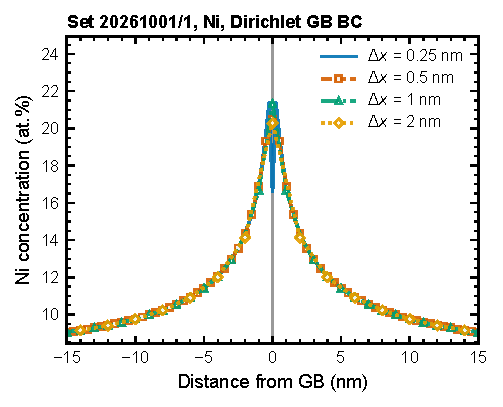
\includegraphics[width=\linewidth]{Ni_Dirich_vs_dx}
  \caption{}\label{fig:Ni-Dirich}
\end{subfigure}\hfill
\begin{subfigure}[t]{0.32\textwidth}\centering
  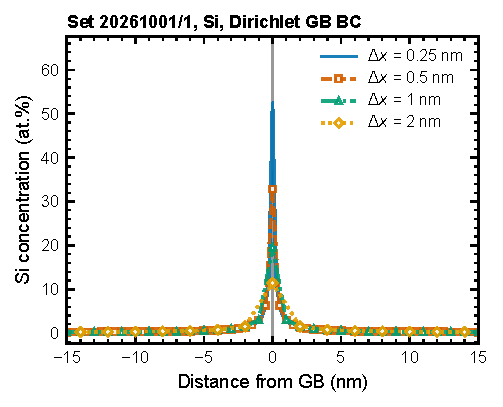
\includegraphics[width=\linewidth]{Si_Dirich_vs_dx}
  \caption{}\label{fig:Si-Dirich}
\end{subfigure}
\par\smallskip
\begin{subfigure}[t]{0.32\textwidth}\centering
  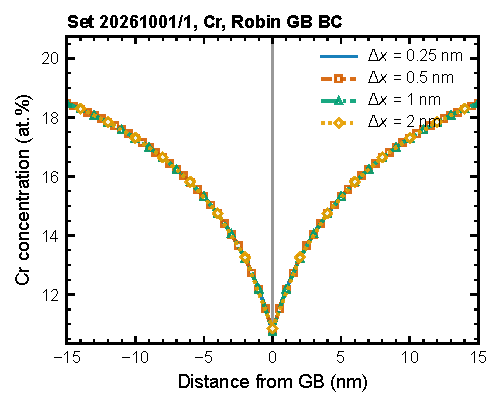
\includegraphics[width=\linewidth]{Cr_Robin_vs_dx}
  \caption{}\label{fig:Cr-Robin}
\end{subfigure}\hfill
\begin{subfigure}[t]{0.32\textwidth}\centering
  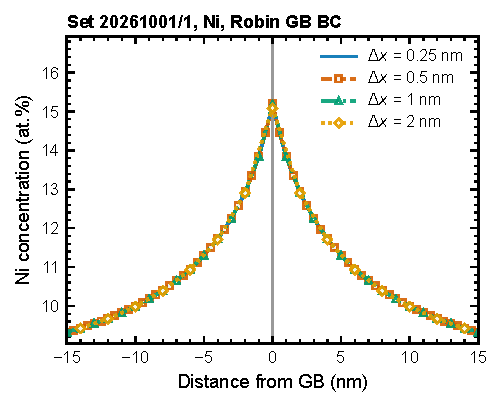
\includegraphics[width=\linewidth]{Ni_Robin_vs_dx}
  \caption{}\label{fig:Ni-Robin}
\end{subfigure}\hfill
\begin{subfigure}[t]{0.32\textwidth}\centering
  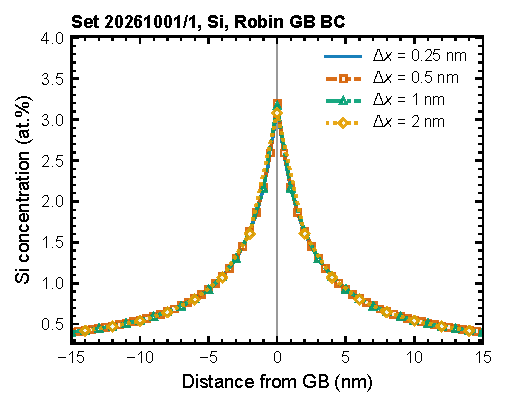
\includegraphics[width=\linewidth]{Si_Robin_vs_dx}
  \caption{}\label{fig:Si-Robin}
\end{subfigure}
\par\smallskip
\begin{subfigure}[t]{0.32\textwidth}\centering
  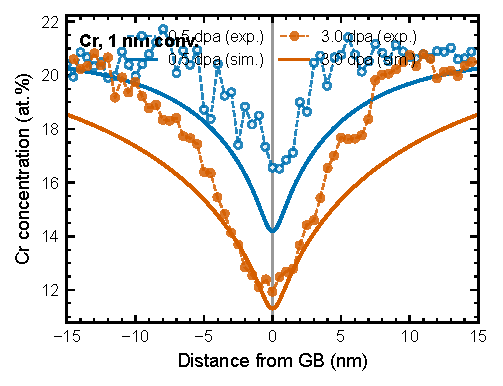
\includegraphics[width=\linewidth]{Cr_doses}
  \caption{}\label{fig:Cr-doses}
\end{subfigure}\hfill
\begin{subfigure}[t]{0.32\textwidth}\centering
  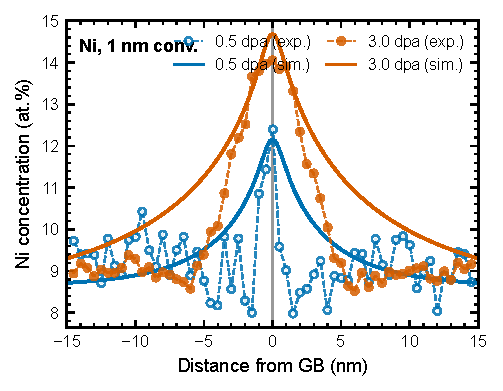
\includegraphics[width=\linewidth]{Ni_doses}
  \caption{}\label{fig:Ni-doses}
\end{subfigure}\hfill
\begin{subfigure}[t]{0.32\textwidth}\centering
  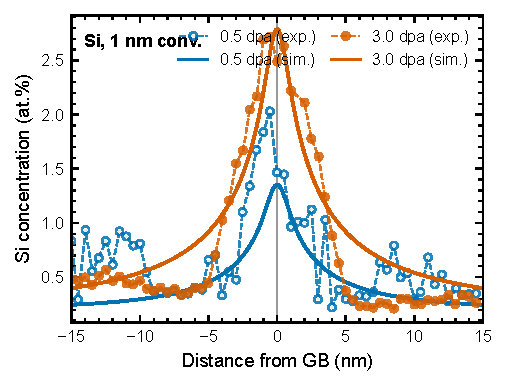
\includegraphics[width=\linewidth]{Si_doses}
  \caption{}\label{fig:Si-doses}
\end{subfigure}
\caption{
Comparison of RIS profiles with Dirichlet BC and Robin BC for GB. (a-c) show the RIS profiles with Dirichlet BC for different mesh sizes. (d-f) show the RIS profiles with Robin BC for different mesh sizes. (g-i) show the RIS profiles with Robin BC for different doses convolved with 1 nm FWHM compared with the experimental data\cite{RN396}.
}
\label{fig:finite-sink}
\end{figure}



In the previous model, the V/I concentration was set to be thermal-equalibrium concentration at the GB, which is a Dirichlet BC indicating the GB is a perfect sink for V/I:
\begin{equation}
C_{\Vac}^{\GB}=C_{\Vac}^{\eq},
\end{equation}
\begin{equation}
C_{\Int}^{\GB}=C_{\Int}^{\eq},
\end{equation}
With this Dirichlet BC, the results are mesh-dependent. With the refinement of the mesh, the defects profiles show a steeper gradient near the GB. Both the gradient and the magnitude of the solute segregation are higher than coarse mesh. Thess results are also observed in other RIS models using Onsager equation. \cite{RN486} 
The width of RIS is also mesh-dependent, and do not converge with mesh refinement. The solution is to use a finite sink for the GB, which is a Robin BC:
\begin{equation}
J_{\Vac}^{\GB}=-k_{\Vac}^{\GB}\left(C_{\Vac}^{\GB}-C_{\Vac}^{\eq}\right),
\end{equation}
\begin{equation}
J_{\Int}^{\GB}=-k_{\Int}^{\GB}\left(C_{\Int}^{\GB}-C_{\Int}^{\eq}\right),
\end{equation}
where $k_{\Vac}^{\GB}$ and $k_{\Int}^{\GB}$ are the sink strength for V/I at the GB. The sink strength and the defect-mediated transport coefficients are calbrated to reproduce both the experimental RIS magnitude and width. 






\printbibliography
\end{document}

